\subsection{Synthetic data}
In this section, we are interested in evaluating the effectiveness of both
MWM and MWMS clustering algorithms by considering different synthetic data generating processes. 
Unless otherwise specified, we set the number of groups $m=50$, number of observations 
per group $n_{j}=50$ in $d=10$ dimensions, number of global clusters $M=5$ with 6 atoms. 
For Algorithm \ref{alg:multilevels_Wasserstein_means} (MWM)
local measures $G_{j}$ have 5 atoms each; for Algorithm \ref{alg:local_constraint_multilevels_Wasserstein_means} (MWMS) number of atoms in constraint set $S_K$ is 50. 
As a benchmark for the comparison we will use a basic 3-stage K-means approach
(the details of which can be found in the Supplement).
The Wasserstein distance between the estimated distributions (i.e. $\hat 
G_1,\ldots,\hat G_m$; $\hat H_1,\ldots,\hat H_M$) and the data generating ones will
be used as the comparison metric. %The details about our comparison metric are deferred to the Supplement.

Recall that the MWM formulation does not impose constraints on the atoms of $G_{i}$,
while the MWMS formulation explicitly enforces the sharing of atoms
across these measures.
We used multiple layers of mixtures while adding Gaussian noise at each layer to generate global and local 
clusters and the no-constraint (NC) data. We varied number of groups $m$ 
from 500 to 10000. We notice that the 3-stage K-means algorithm performs the best 
when there is no constraint structure \emph{and} variance is constant across clusters (Fig. 
\ref{fig:simul_M}(a) and \ref{fig:simul_N}(a)) --- this is, not surprisingly, a favorable setting for the basic K-means method.
As soon as we depart from the (unrealistic) constant-variance, no-sharing assumption, both of our
algorithms start to outperform the basic three-stage K-means.
The superior performance is most pronounced with local-constraint (LC) data (with or without constant variance conditions). 
See Fig. \ref{fig:simul_M}(c,d).
It is worth noting that even when group variances are constant, the 3-stage K-means is no longer
longer effective because now fails to account for the shared structure. 
When $m=50$ and group sizes are larger, we set $S_K=15$. Results are reported in 
Fig. \ref{fig:simul_N} (c), (d). 
These results demonstrate the effectiveness and flexibility of our both algorithms.

%The MWMS, on the other hand, encourages the sharing of atoms across local barycenters. 
%We again use multiple layers of mixtures with Gaussian noise, and
%enforce atom-sharing among groups to generate local-constraint (LC) data. 
%Fig. \ref{fig:simul_M} (c) and (d) demonstrates superior performance of the MWMS clustering
%algorithm over both MWM algorithm and the baseline 3-state K-means clustering method.

\subsection{Real data analysis} 
\begin{figure*}[t]
\begin{centering}
\subfloat[\label{fig:labelme_clusters}]{\begin{centering}
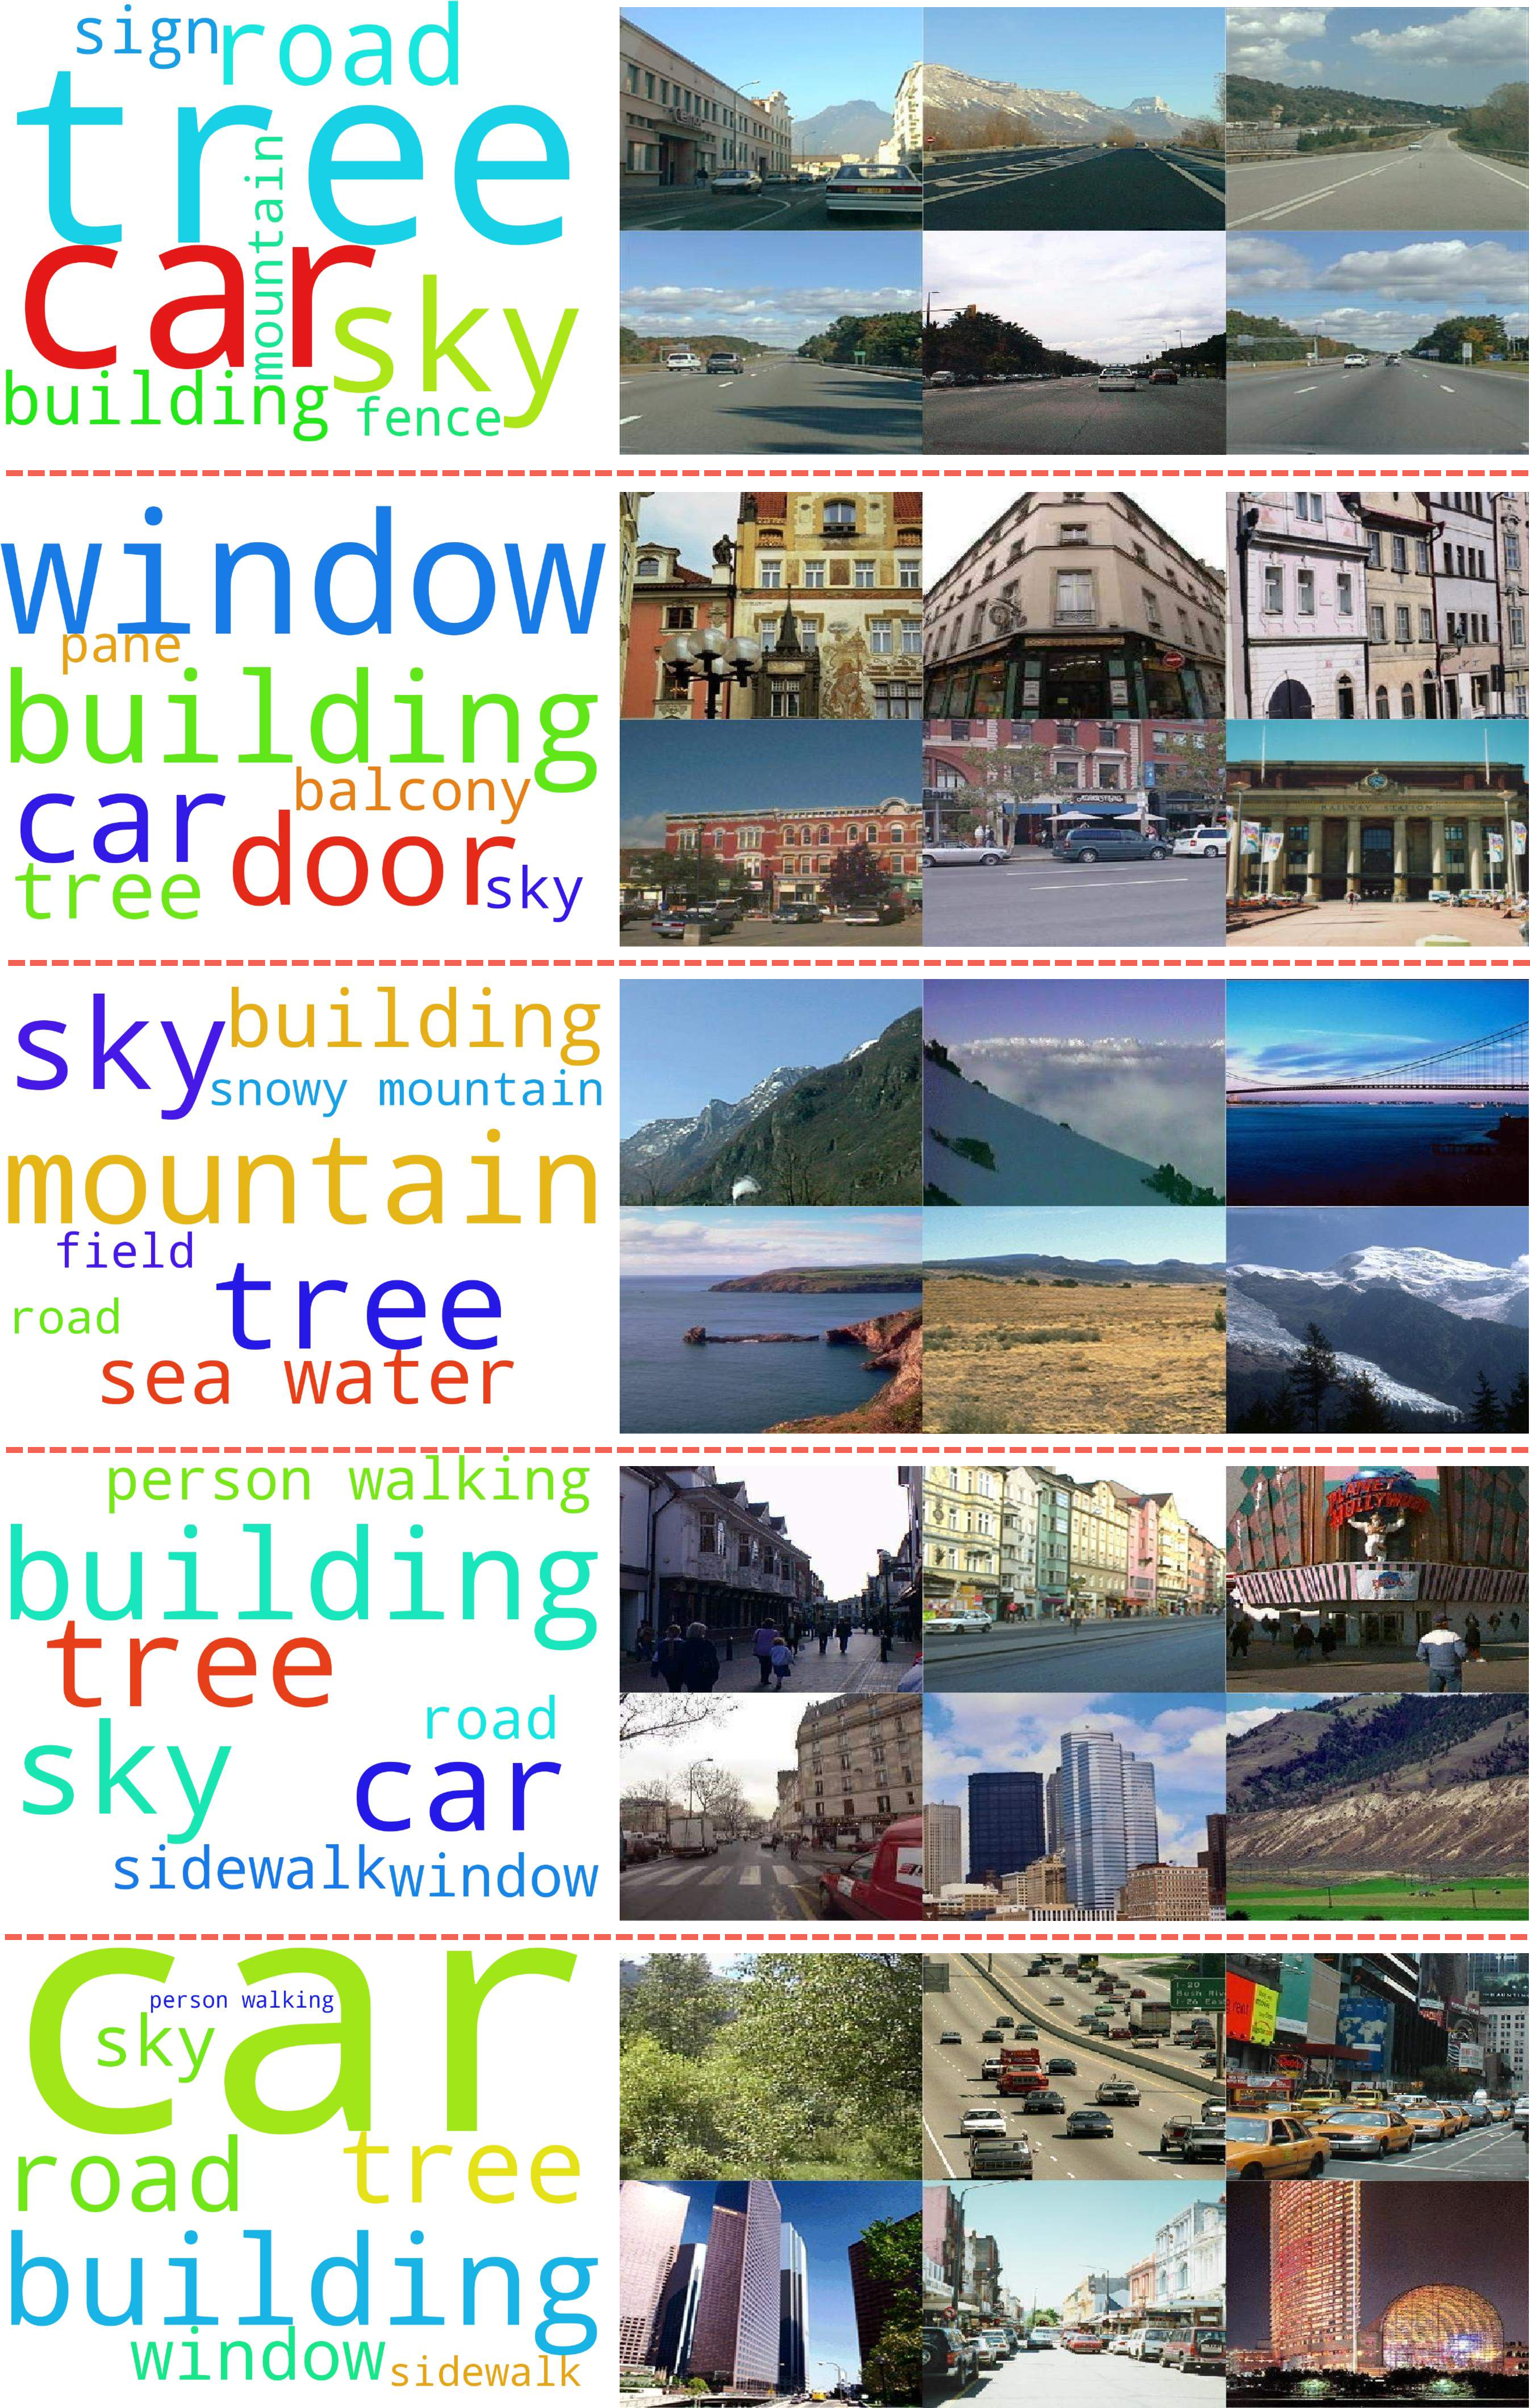
\includegraphics[width=0.2\paperwidth]{top5topics_old_compressed}
\par\end{centering}

}\qquad{}\subfloat[
\label{fig:SL-graph}
]{\begin{centering}
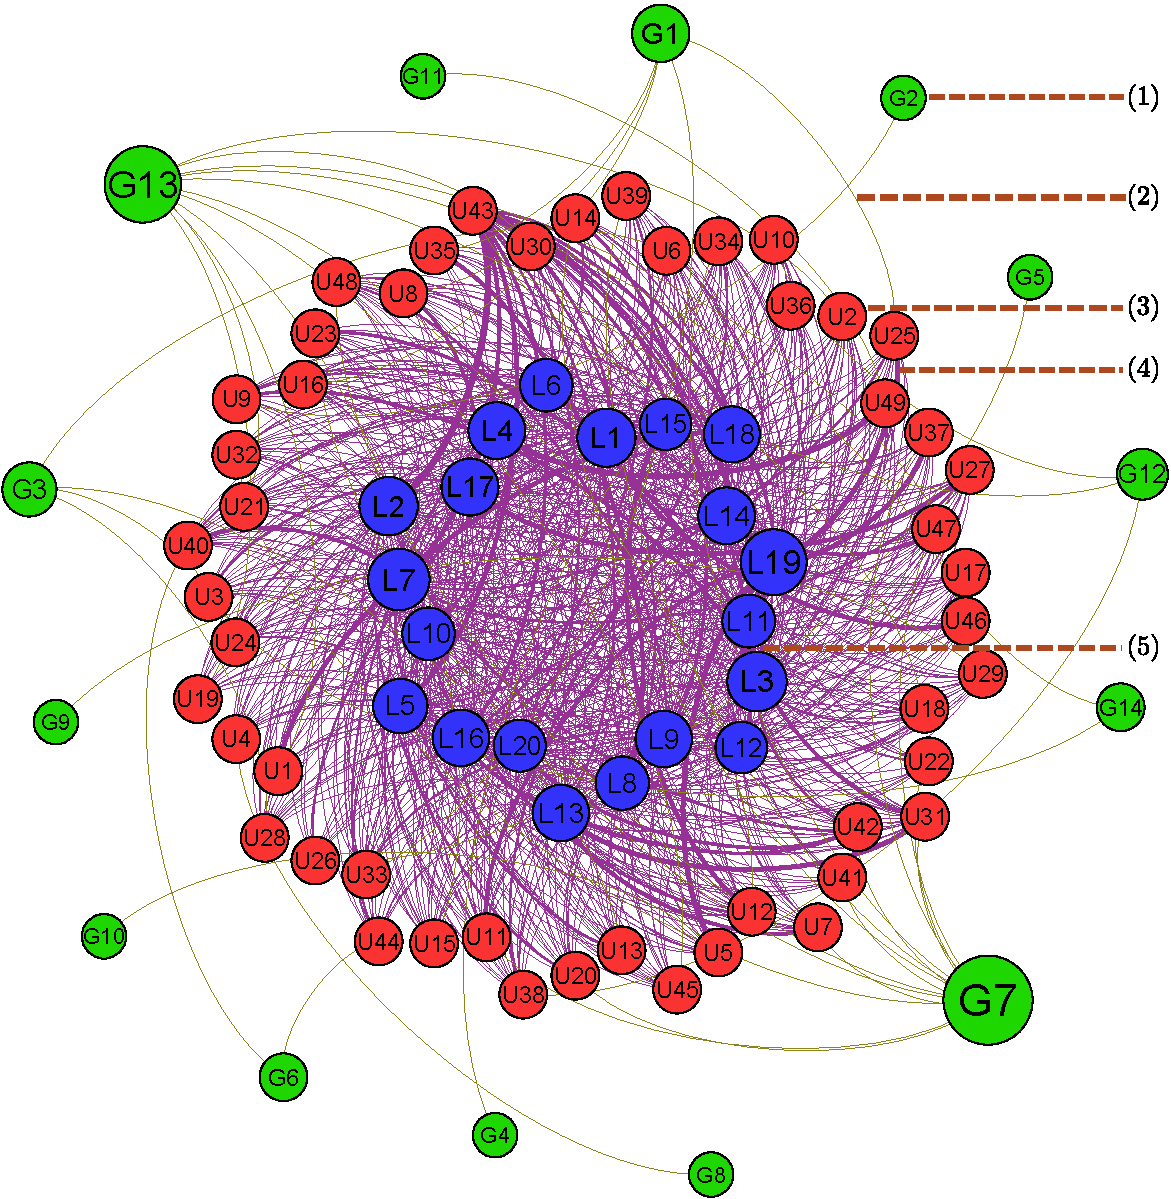
\includegraphics[width=0.3\paperwidth]{SL_graph_new_new}
\par\end{centering}

}
\par\end{centering}

\caption{
Clustering representation for two datasets: (a) Five image clusters
from \emph{Labelme} data discovered by MWMS algorithm: tag-clouds
on the left are accumulated from all images in the clusters while
six images on the right are randomly chosen images in that cluster;
(b) StudentLife discovered network with three node groups: (1) discovered
student clusters, (3) student nodes, (5) discovered activity location
(from Wifi data); and two edge groups: (2) Student to cluster assignment,
(4) Student involved to activity location. Node sizes (of discovered
nodes) depict the number of element in clusters while edge sizes between
\emph{Student} and \emph{activity location }represent the popularity
of student's activities.
}
\end{figure*}

We applied our multilevel clustering algorithms to two real-world datasets: LabelMe and StudentLife.

\textbf{LabelMe dataset} consists of $2,688$ annotated
images which are classified into 8 scene categories including \emph{tall
buildings, inside city, street, highway, coast, open country, mountain,}
and \emph{forest} \cite{Oliva-2001} . Each image contains multiple
annotated regions. Each region, which is annotated by users, represents
an object in the image.  As shown in Figure \ref{fig: LabelMeExample}, the left
image is an image from \emph{open country }category and contains
4 regions while the right panel denotes an image of \emph{tall buildings}
category including 16 regions. Note that the regions in each image can
be overlapped. We remove the images containing less then 4 regions
and obtain $1,800$ images. 

\begin{figure}
\centering{}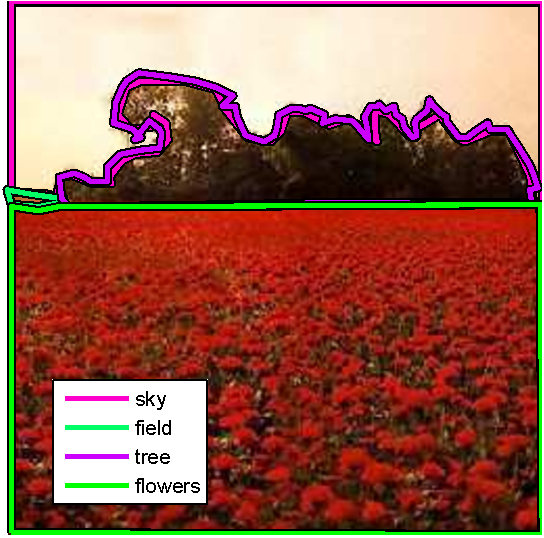
\includegraphics[width=0.17\textwidth]{LabelMeSample_new}\qquad{}\qquad{}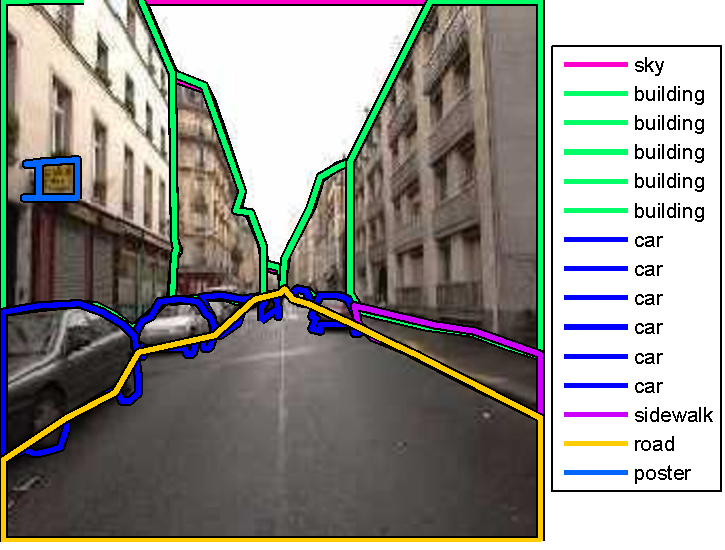
\includegraphics[width=0.22\textwidth]{LabelMeSample2_new}\caption{Examples of images used in LabelMe dataset. Each image consists of
different annotated regions.\label{fig: LabelMeExample}}
\end{figure}

We then extract GIST feature \cite{Oliva-2001} for each region in a image.
GIST is a visual descriptor to represent perceptual dimensions and
oriented spatial structures of a scene. Each GIST descriptor is a
512-dimensional vector. We further use PCA to project GIST features
into 30 dimensions. Finally, we obtain $1,800$ ``documents'', each
of which contains regions as observations. Each region now is represented
by a 30-dimensional vector. We now can perform clustering regions
in every image since they are visually correlated. In the next level
of clustering, we can cluster images into scene categories.
\begin{table}
\caption{Clustering performance for LabelMe
dataset.}
\label{tab:clustering_metrics}
\centering
\begin{tabular}{lcccc}
%\hlin%e 
\toprule
Methods & \textcolor{black}{NMI} & ARI & \textcolor{black}{AMI} & \textcolor{black}{Time (s) } \\
%\hline 
%\hline 
\midrule
\textcolor{black}{K-means} & 0.349 & 0.237 & 0.324 & \textbf{0.3}\\
TSK-means & 0.236 & 0.112 & 0.22 & 218\\
%\hline 
MC2 & 0.315 & 0.206 & 0.273 & 4.2\\
%\hline 
\textbf{\textcolor{black}{MWM}} & 0.373 & 0.263 & 0.352 & 332 \\
%\hline 
\textbf{MWMS} & \textbf{0.391} & \textbf{0.284} & \textbf{0.368} & 544 \\
%\tabularnewline
%\hline 
\bottomrule
\end{tabular}
\end{table}

\comment{
\begin{table}
\begin{centering}
\begin{tabular}{|c|c|c|c|c|}
\hline 
Methods & \textcolor{black}{NMI} & ARI & \textcolor{black}{AMI} & \textcolor{black}{Time (s) }\tabularnewline
\hline 
\hline 
\textcolor{black}{K-means} & 0.349 & 0.237 & 0.324 & \textbf{0.3}\tabularnewline
\hline 
TSK-means & 0.236 & 0.112 & 0.22 & 218\tabularnewline
\hline 
MC2-SVI & 0.315 & 0.206 & 0.273 & 4.2\tabularnewline
\hline 
\textbf{\textcolor{black}{MWM}} & 0.373 & 0.263 & 0.352 & 332 \tabularnewline
\hline 
\textbf{MWMS} & \textbf{0.391} & \textbf{0.284} & \textbf{0.368} & 544 \tabularnewline
\hline 
\end{tabular}
\par\end{centering}

\caption{\label{tab:clustering_metrics}Clustering performance for LabelMe
dataset.}
\end{table}}


\textbf{StudentLife dataset} is a large dataset frequently
used in pervasive and ubiquitous computing research. Data signals consist of
multiple channels  (e.g., WiFi signals, Bluetooth scan, etc.), which are
collected from smartphones of 49 students at Dartmouth
College over a 10-week spring term in 2013. However, in our experiments,
we use only WiFi signal strengths. We applied a similar procedure
described in \cite{nguyen_nguyen_venkatesh_phung_icpr16mcnc} to pre-process the
data. We aggregate the number of scans by each Wifi access point and
select 500 Wifi Ids with the highest frequencies. Eventually, we obtain
49 ``documents'' with totally approximately $4.6$ million 500-dimensional
data points.

\textbf{Experimental results.} To quantitatively evaluate our proposed
methods, we compare our algorithms with several base-line methods:
K-means, three-stage K-means (TSK-means) as described in the Supplement, 
MC2-SVI without context \cite{Viet-2016}. Clustering performance in Table
\ref{tab:clustering_metrics} is evaluated with the image clustering
problem for \emph{LabelMe dataset}. With \emph{K-means}, we
average all data points to obtain a single vector for each images.
K-means needs much less time to run since the number of data points
is now reduced to $1,800$. For MC2-SVI, we used stochastic varitational and 
a parallelized Spark-based implementation in \cite{Viet-2016} to carry out 
experiments. This implementation has the advantage of making use of all of 16 cores on the test machine. 
The running time for MC2-SVI is reported after scanning one epoch.
In terms of clustering accuracy, MWM and MWMS algorithms 
perform the best.

Fig. \ref{fig:labelme_clusters} demonstrates five representative
image clusters with six randomly chosen images in each (on the right)
which are discovered by our MWMS algorithm. We also accumulate labeled
tags from all images in each cluster to produce the tag-cloud on the
left. These tag-clouds can be considered as visual ground truth of
clusters. Our algorithm can group images into clusters which are consistent
with their tag-clouds.

We use StudentLife dataset to demonstrate the capability of multilevel
clustering with large-scale datasets. This dataset not only contains
a large number of data points but presents in high dimension. Our
algorithms need approximately 1 hour to perform multilevel
clustering on this dataset. Fig. \ref{fig:SL-graph} presents two
levels of clusters discovered by our algorithms. The innermost (blue)
and outermost (green) rings depict local and global clusters respectively.
Global clusters represent groups of students while local clusters
shared between students (``documents'') may be used to infer
locations of students' activities. From these clusteing we can dissect
students' shared location (activities), e.g. Student 49 (\emph{U49})
mainly takes part in activity location 4 (\emph{L4}). 
